\documentclass[11pt,a4]{article} 
\usepackage[ansinew]{inputenc} %Schrifttyp und Umlaute
\usepackage{epsfig} %Nutzung von eps files
%\usepackage[dvips]{epsfig} %Nutzung von eps files
%\usepackage[final]{graphicx}    
%\usepackage[off]{auto-pst-pdf}     % necessary for psfrag to work
\usepackage{epstopdf} 

\usepackage[bf,sf,compact]{titlesec} 
\usepackage{fancyhdr} 
\usepackage{amsmath}
\usepackage{amssymb} %Symbole nach AMS
\usepackage{amstext}
\usepackage{theorem}
\usepackage{subfigure}
\usepackage{booktabs}

\usepackage{flafter}
\usepackage{exscale}
\usepackage{float}   % for minipages
\usepackage{psfrag}


\setlength{\parindent}{0cm} 
\setlength{\textwidth}{16cm}
\setlength{\oddsidemargin}{0cm}  
\setlength{\voffset}{-2,8cm}  
\setlength{\textheight}{25cm} 
\setlength{\arrayrulewidth}{0,3mm} 
\setlength{\textheight}{25cm} 

\renewcommand{\labelenumi}{\alph{enumi})} 
\sloppy



\begin{document} %hier geht es los

\thispagestyle{empty} 
\begin{tabular*}{16cm}{lr} \hline \\ %Tabelle mit zwei Spalten, in jeder Spalte eine minipage, neue Zeile mit \\
    \begin{minipage}{10cm} %Anfang minipage in linker Spalte, Breite 8cm
            \textsf{Technische Universit\"at Dortmund \\ %Schriftgröße smallface
            Department of Biochemical and Chemical Engineering \\
            Chair of Process Dynamics and Operations \\
            Prof.~Dr.~Sebastian Engell \\}
    \end{minipage} & %Ende minipage in linker Spalte
    \begin{minipage}{6cm} %Anfang minipage in rechter Spalte, Breite 8cm
            \setlength{\unitlength}{1cm} %Formatierung, Platzierung und Einfuegen des ASTLOGOS
            \begin{picture}(8,1) 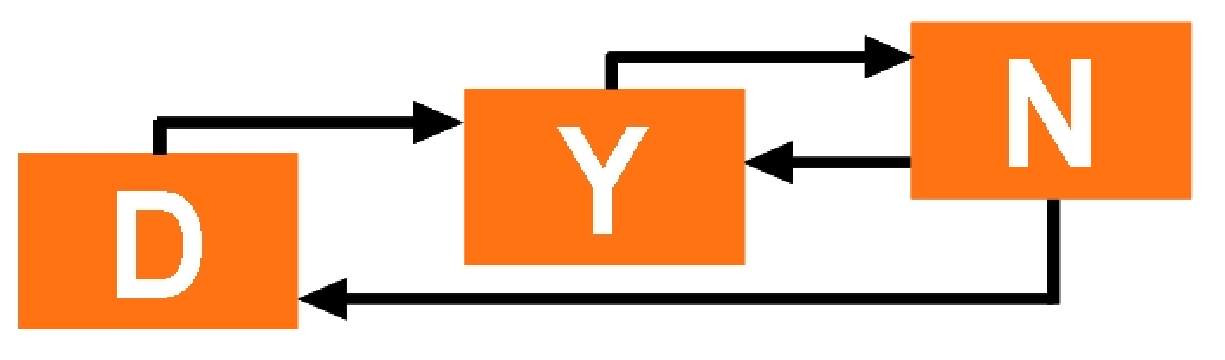
\epsfig{file= Astlogo.eps, width=5cm}
            \end{picture}\par
    \end{minipage} \\ \hline %Ende minipage in rechter Spalte
\end{tabular*} %Ende Tabelle




\vspace{5cm}

\begin{center} 

\LARGE{\bfseries EXAMPLE TITLE \\

    Automation \& Robotics 
    
    Group Project SS18 \\}
\end{center}



%%%%%%%%%%%%%%%%%%%%%%%%%%%%
\clearpage
\titleformat{\section}{\Large\bf}{\thesection:}{20pt}{}
\setcounter{enumi}{0} \section*{Abstract} %

\subsection*{Introduction}
The pipe-less plant at the Process Dynamics and Operations group is an experimental setup of Automated Guided Vehicles (AGVs) moving between various stations. The AGVs dynamically change trajectories in operational mode based on a Model Predicative Control (MPC) scheme with the objective to get from one station to the other while at the same time avoiding each other. The current positioning system is based on pattern recognition where the system tracks each AGV based on a unique pattern of LEDs via a camera that overlooks the plant. 
\subsection*{Motivation for new positioning system
}
The vision based positioning system displays some flaws and should be replaced by a system more adapted to the actual operational environment of the experimental plant. The following problems have been identified in the current setup of the system: 

\begin{itemize}
	\item No position feedback in bright day-light conditions 
	\item A ``\textit{fish-eye camera lense problem}'', meaning that the position error grows with the distance from the center of the image caused by the distortion a wide angle lense creates
	\item Problems related to the software implementation restricting the usage of incoming information from the camera
\end{itemize}

\subsection*{Project objective
}
The project aimed at first evaluating different potential positioning systems, selecting one of them based on defined metrics and then to develop a proof-of-concept based on the chosen technology for the experimental pipe-less production plant in a model driven fashion. After going through four different alternatives including a triangulation based methods for indoor applications, another pattern recognition based method (such as QR-codes), map-based localization, and Radio-Frequency Identification (RFID), the latter was chosen for further evaluation and implementation.
\subsection*{Theoretical Background}
RFID is a versatile technology with multiple application areas, e.g. access control, race tracking and positioning. Automated multi-agent systems are increasingly utilizing RFID for localization as the technology has been proven to have many advantages over vision based positioning systems.It uses electromagnetic fields to automatically identify and track tags attached to objects. There are two potential ways to implement an RFID localization system. One option is based on active RFID transmitters and reader with wide coverage areas that can be placed along the edges of the plant area and on each AGV. The other option is based on comparatively many passive tags, uniformly placed, on the ground of the plant area and active readers on the AGVs. The latter option was chosen for the project based on cost efficiency, system scalability and from literature proven applicability.
\subsection*{Hardware
}
An RFID system is made up of two parts: a tag and a reader. RFID tags are embedded with a transmitter and a receiver. The RFID component on the tags has two parts: a microchip that stores and processes information, and an antenna to receive and transmit a signal, which partly contains the unique ID of the tag. The hardware components which are added to the AGVs comprise an RFID antenna, an RFID reader and a WiFi module. All the devices are supplied with 5V. The antenna is connected to the reader via a coaxial so called ``\textit{SubMiniature version A}''(SMA) cable and the reader communicates via an RX/TX interface. The RFID reader and the WiFi-module are connected via wired serial communication. The WiFi module then transmits the reader data through the local network, using TCP/IP communication. The system data is lastly received by a PC that represents the control hub of the plant through a framework implemented in C Sharp (C\#). 
\subsection*{Communication
}
The WiFi-Module is connected to the same router as the PC on which the system user interface is running. A TCP-Client was established in the C\# framework in order to handle incoming RFID data. The WiFi-module continuously sends data and the algorithm calculating AGV position prompts for this data as position and/or orientation of an AGV needs to be computed.
\subsection*{Localization
}
The implemented positioning algorithm requires the ID and the received signal strength indication (RSSI) of at least three RFID tags to calculate the position of the antenna. The RSSI gives a relation between the detected tag and the distance to it, in other words, a radius. The system has a record of the position of each tag and the ID of each tag hence holds information about the uniquely defined position of the tag. With three positions and the three corresponding radii, one can use trilateration to compute the position of the antenna.  
\subsection*{Initialization Procedure
}
Initially the system cannot  know the orientation of the AGV even if it can read enough RFID tags, as the tags only provide the x and y coordinates of the antenna itself (which is located off center on the robot). The main goal of the initializing procedure is to estimate both the starting position and orientation. During the turn, the robot will make a short stop every 45° and estimate the position of the antenna at that point. At the end of the procedure, the algorithm calculates the center of the eight recorded points. It takes two positions plus their corresponding positions at the other side (plus 180$^{\circ}$) and computes the intersection of the linear function which goes through the position and its corresponding point. To estimate the orientation the algorithm computes the angle between the estimated position and the position of the antenna at 360$^{\circ}$/0$^{\circ}$. 
\subsection*{Demonstrator and results}
A proof-of-concept for an RFID based localization system has been built in a model-driven fashion. The new system was simulated using Matlab to evaluate its applicability and overcome engineering problems at an early stage of the design phase. An initialization algorithm has been designed and implemented to calculate the starting position and heading of the robot.  Simulations show an average position error of 0.5 cm. Analogously, the orientation of an error of around 10$^{\circ}$. The system prototype consists of a reader and an area of nine tags (3x3).  The measured position error in the experimental setup was on average 2.5 cm. The error of the orientation was on average about 23$^{\circ}$. This significant difference to simulated results was caused by two main reasons: Firstly, some tags could not be detected by the reader. Secondly, the test board was quite small as it consisted of so few RFID tags which meant that it was not representative enough of the intended design. To summarize, it can be said that on the one hand a rather low-cost, scalable solution was designed which can work in any area independent for any light conditions.  On the other hand, the accuracy of the technology is not very reliable according to the experiments made. This can be improved in further work with a better system setup and an improved localizing algorithm.



%%%%%%%%%%%%%%%%%%%%%%%%%%%%
\clearpage
\tableofcontents


\setlength{\textheight}{20cm}

\pagestyle{fancy} 
\lhead{Final report, TITLE, DD.MM.YYYY}
\chead{}
\rhead{Page \thepage}
\lfoot{}
\cfoot{}
\rfoot{} 
\renewcommand{\headrulewidth}{0.4pt} 

\setlength{\topmargin}{2cm} %oberer Rand bis Oberkante Kopfzeile

\makeatletter \def\usecounter#1{\@nmbrlisttrue\def\@listctr{#1}}
\makeatother 
\setcounter{figure}{0}
\setcounter{table}{0} 


%%%%%%%%%%%%%%%%%%%%%%%%%%%%
\titleformat{\section}{\Large\bf}{\thesection}{20pt}{}
\section{Introduction} %

Add your name to the file name



%%%%%%%%%%%%%%%%%%%%%%%%%%%%
\clearpage
\titleformat{\section}{\Large\bf}{\thesection}{20pt}{}
\section{Theory} %

\begin{itemize}
\item Example
\item 
\end{itemize}



\label{LetzteSeite} %marker letzte Seite


\end{document}

\label{LetzteSeite} %marker letzte Seite
